\section{CPLD-based mouse control}
A small CPLD (Altera EPM7032) has been used to interface with a mouse's buttons. The Quartus II IDE has been used for design synthesis and the device has been programmed using a BusPirate serial interface together with OpenOCD.

From an external point of view, the three mouse's buttons change the position reference of the levitating object: when button 1 (left) is pressed, the position of the object is decreased (the object goes down). When button 2 (right) is pressed, the position is increased (the object goes up), while when button 3 (center) is pressed the position is reset to the initial value.

Electrically, the buttons are seen as simple switches, with a built-in forward-biased protection diode. This makes it impossible to feed them with 3.3V inputs, as the output would be lowered to 2.7V. So, the 5V rail is used as an input for the buttons, which close to pull-down networks made of a 100$\Omega$ resistor in serie with a 3.3V zener diode and a 10K$\Omega$ resistor. When the switch is open, the two resistor act as a single pull-down resistor and bring the output to 0V. When the button is pressed, the zener diode in serie with the 100$\Omega$ resistor regulates the output voltage to 3.3V, which is a correct value for the input pins of the CPLD.

The CPLD is in charge of constantly sampling the button adjusting the reference position and communicating it to the microcontroller. The reference value is kept in memory and communicated divided by 16 (i.e. last 4 bits are omitted and set to 0). For BTN1 and BTN2 inputs, two flip-flops in series keep track of the current and previous value of the line. An OR port between these gates decides whether at least one of the buttons have been pressed. The current reference value is kept into an 8-bit register, whose clock signal is the falling edge of the latter OR gate's output. In this way, the register is updated when buttons are released. The register outputs both to the external pins of the CPLD (connected in parallel to the microcontroller) and to an 8-bit adder. The other input for the adder can be +1 or -1, and is multiplexed using the previous value of BTN1 as a selection signal. The output of the adder loops back to the register's input. In this way, if button 1 has just been released, the value "1" is added to the current register's value; on the other hand, if button 1 has not been released, this means the released button was button 2, and so "-1" is added to the current value.

On the loopback track between the summer's output and the register's input another multiplexer is present: this is used to avoid overflow or underflow of the value. If the value is too high to be incremented more, and button 1 has been released, or the value is too low to be decremented, and button 2 has been released, the output of the summer is bypassed and substituted with the actual register's value. In this way, the register can't increase its value to be more than or less than predefined limits (0xFF for overflow, 0x0F for underflow). When overflow or underflow occour, LEDs are turned on the main board to signal the event.

The buttons are sampled at a low rate (25Hz), which clock signal is generated by an external LM555-based oscillator. This low rate is necessary to also implement debouncing of the buttons.

An OR gate between button 3 and an external reset line (connected to the microcontroller for initialization) is used as an asynchronous reset signal for the CPLD.

Full-behavioural implementation of this architecture required more macrocells than available on the CPLD (34/32), but with a few optimizations it has been fitted into the 32 macrocells. At the end a more compact, RTL implementation has been chosen which resulted in a good optimization requiring 21/32 macrocells.

\begin{figure}[htbp]
\centering
\includegraphics[width=6in]{Graphics/mouseSchema}
\caption{Schema of the digital circuit implemented into the CPLD.}
\end{figure}

\begin{figure}[htbp]
\centering
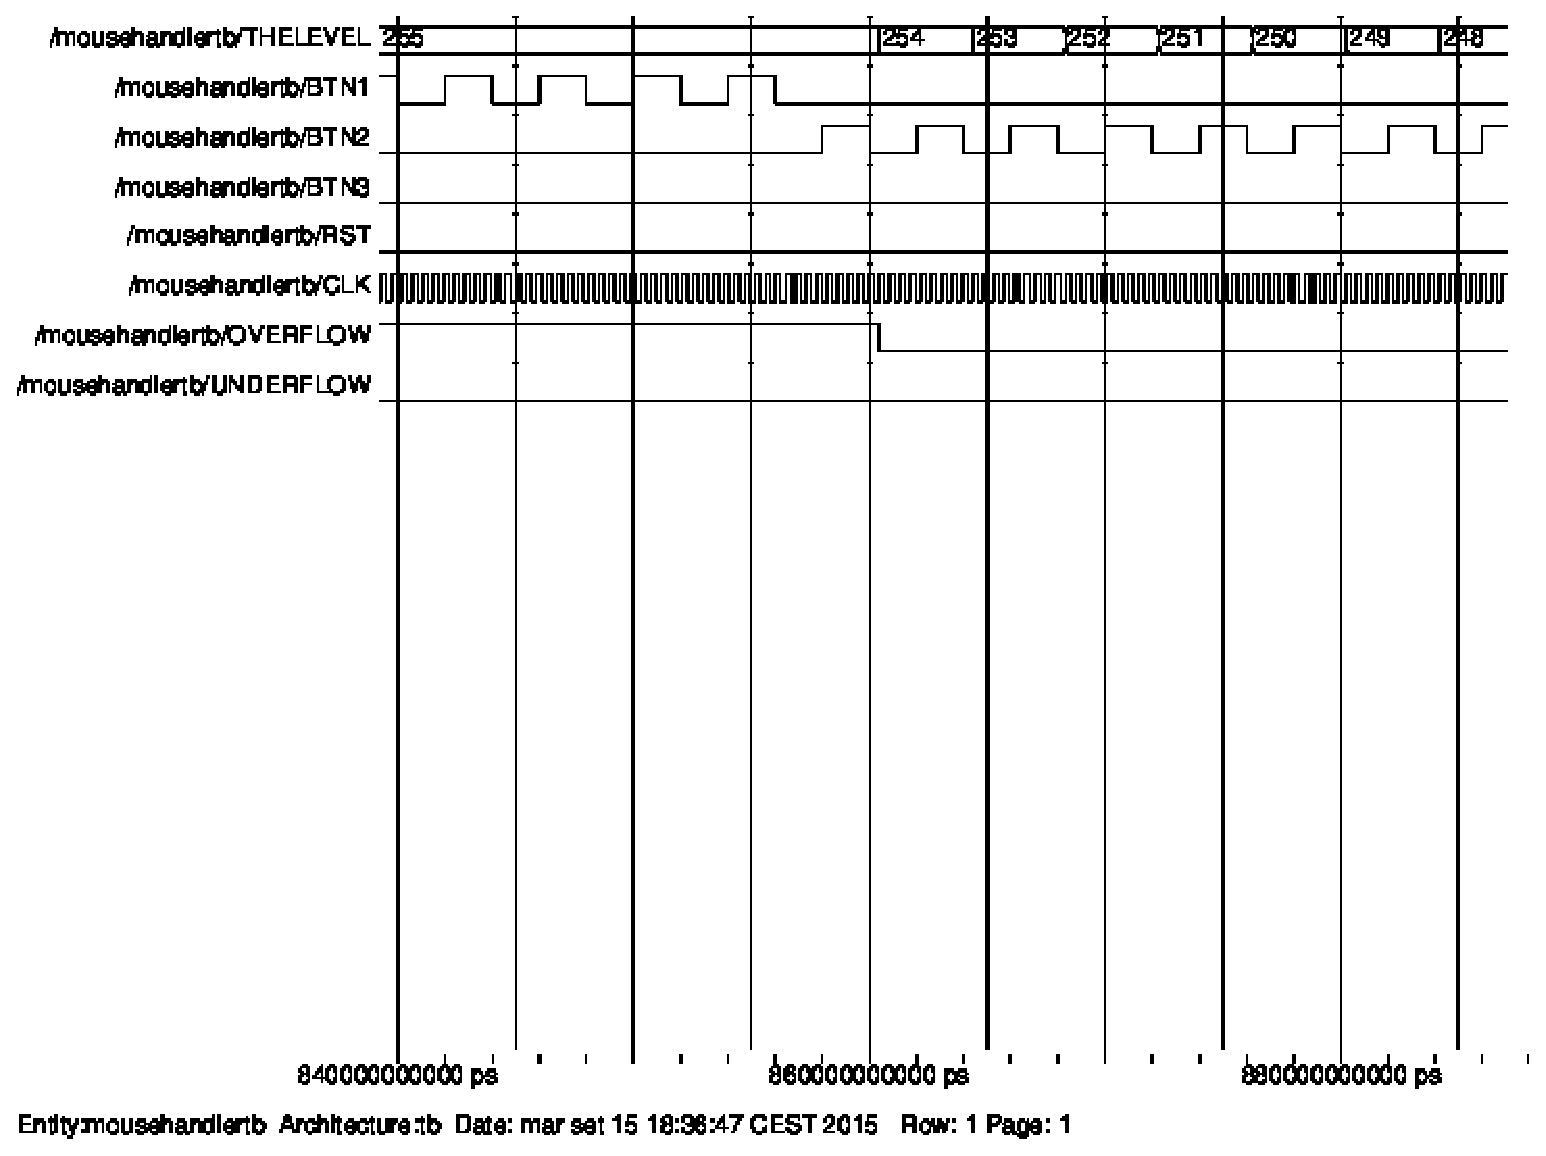
\includegraphics[width=4in]{Graphics/mouseOFW}
\caption{When the upper limit for the value is reached, it is not possible to increase it anymore and the corresponding "overflow" line is actived. Pressing button 2 to decrease the value corrects the problem and changes the value accordingly.}
\end{figure}

\begin{figure}[htbp]
\centering
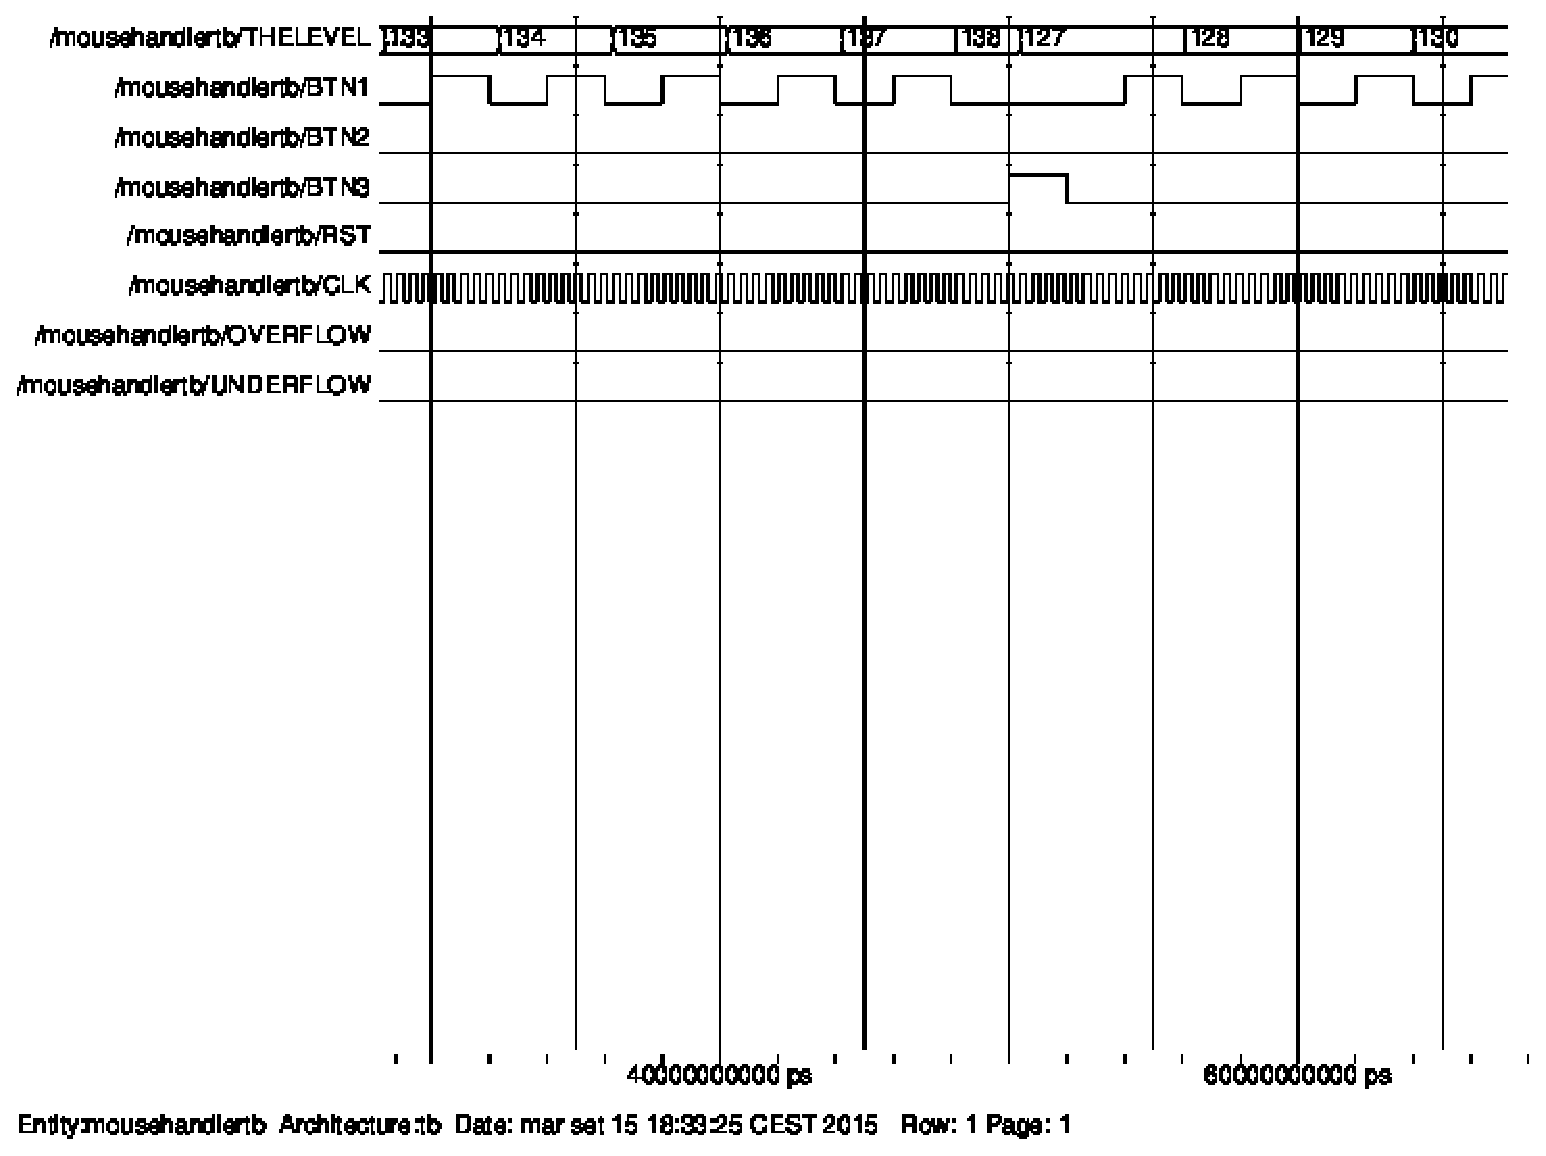
\includegraphics[width=4in]{Graphics/mouseRST}
\caption{Button 3 acts as an asynchronous reset for the stored value}
\end{figure}




